\documentclass[abstracton]{scrartcl}
\usepackage{myOptions}
\usetikzlibrary{external}
\tikzexternalize % activate

\tikzset{
    png export/.style={
        external/system call=%
        {xelatex \tikzexternalcheckshellescape -halt-on-error -interaction=batchmode -jobname "\image" "\texsource";%
         convert -density 300 -transparent white "\image.pdf" "\image.png"; rm -f "\image.pdf"},
    }
}

\tikzset{%
    % Add size information to the .dpth file (png is in density not size)
    /pgf/images/external info,
    % Use the png export AND the import
    use png/.style={png export,png import},
    png import/.code={%
        \tikzset{%
            /pgf/images/include external/.code={%
                % Here you can alter to whatever you want
                % \pgfexternalwidth is only available if /pgf/images/external info
                % is set
                \includegraphics%
                [width=\pgfexternalwidth,height=\pgfexternalheight]%
                {{##1}.png}%
            }%
        }%
    }%
}


\begin{document}

\bgroup \tikzset{png export} 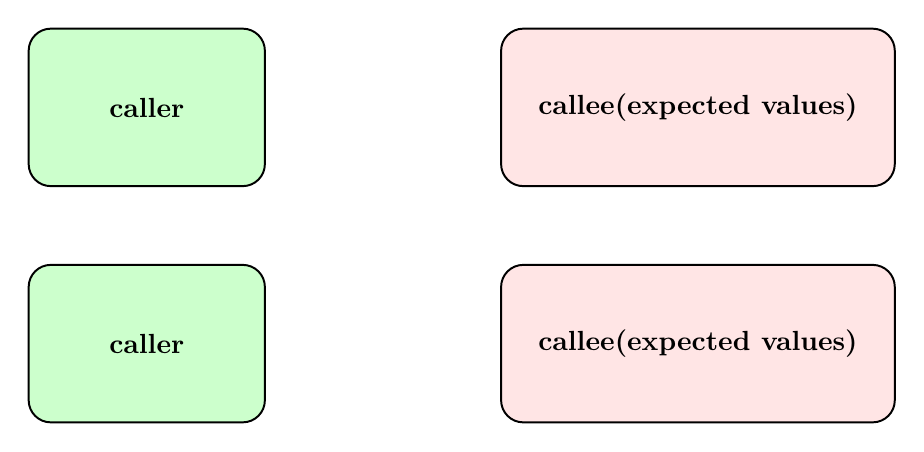
\begin{tikzpicture}
\draw [fill = green!20!white, rounded corners = 8pt, line width = 0.25mm]  (0,0) rectangle (3,2) node[pos=.5] {\textbf{caller}};
\draw [fill = red!10!white, rounded corners = 8pt, line width = 0.25mm]  (6,0) rectangle (11,2) node[pos=.5] {\textbf{callee(expected values)}};
\arrow{startX=3,startY=1,endX=6,endY=1, label=\textbf{passed values}}
\draw [fill = red!10!white, rounded corners = 8pt, line width = 0.25mm]  (6,-3) rectangle (11,-1) node[pos=.5] {\textbf{callee(expected values)}};
\draw [fill = green!20!white, rounded corners = 8pt, line width = 0.25mm]  (0,-3) rectangle (3,-1) node[pos=.5] {\textbf{caller}};
\arrow{startX=6,startY=-2,endX=3,endY=-2, label=\textbf{<return value>}, style=dashed, aboveBelow=below}
\end{tikzpicture} \egroup

\vskip 2cm

Example 1 

\vskip 2cm

\bgroup \tikzset{png export} 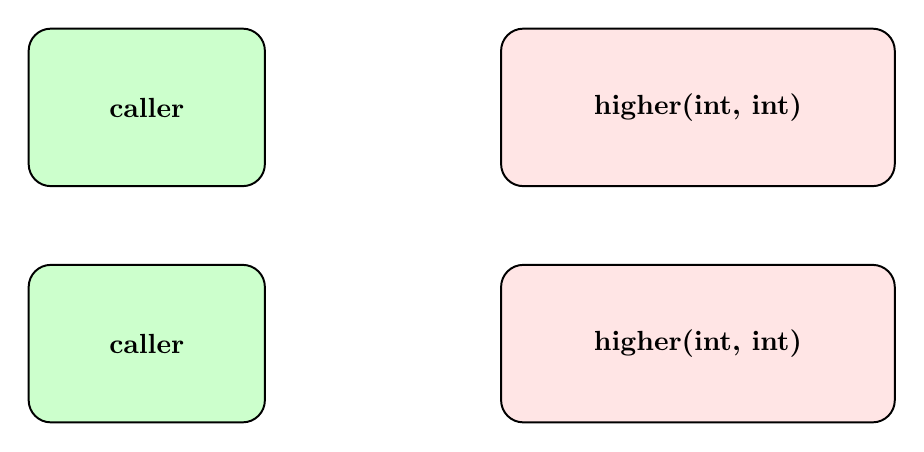
\begin{tikzpicture}
\draw [fill = green!20!white, rounded corners = 8pt, line width = 0.25mm]  (0,0) rectangle (3,2) node[pos=.5] {\textbf{caller}};
\draw [fill = red!10!white, rounded corners = 8pt, line width = 0.25mm]  (6,0) rectangle (11,2) node[pos=.5] {\textbf{higher(int, int)}};
\arrow{startX=3,startY=1,endX=6,endY=1, label=\textbf{2, 5}}
\draw [fill = red!10!white, rounded corners = 8pt, line width = 0.25mm]  (6,-3) rectangle (11,-1) node[pos=.5] {\textbf{higher(int, int)}};
\draw [fill = green!20!white, rounded corners = 8pt, line width = 0.25mm]  (0,-3) rectangle (3,-1) node[pos=.5] {\textbf{caller}};
\arrow{startX=6,startY=-2,endX=3,endY=-2, label=\textbf{5}, style=dashed, aboveBelow=below}
\end{tikzpicture} \egroup

\vskip 2cm

Example 2

\vskip 2cm

\bgroup \tikzset{png export} 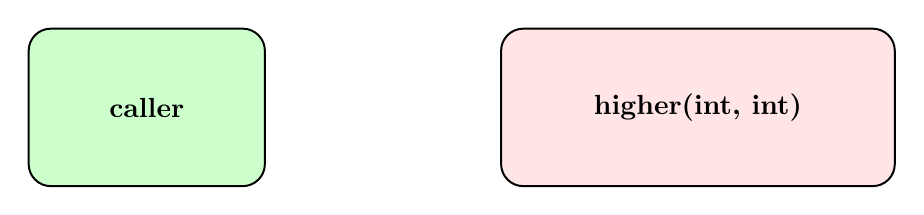
\begin{tikzpicture}
\draw [fill = green!20!white, rounded corners = 8pt, line width = 0.25mm]  (0,0) rectangle (3,2) node[pos=.5] {\textbf{caller}};
\draw [fill = red!10!white, rounded corners = 8pt, line width = 0.25mm]  (6,0) rectangle (11,2) node[pos=.5] {\textbf{higher(int, int)}};
\arrow{startX=3,startY=1,endX=6,endY=1, label=\textbf{\textcolor{red}{15}}}
\arrow{colour=red, arrowheadsize=0.01, startX=3,startY=2,endX=6,endY=-1, label=\textbf{too few parameters}, style=dashed, aboveBelow=below}
\arrow{colour=red, arrowheadsize=0.01, startX=3,startY=-1,endX=6,endY=2, style=dashed, aboveBelow=below}
\end{tikzpicture} \egroup


\vskip 2cm

Example 3

\vskip 2cm

\bgroup \tikzset{png export} 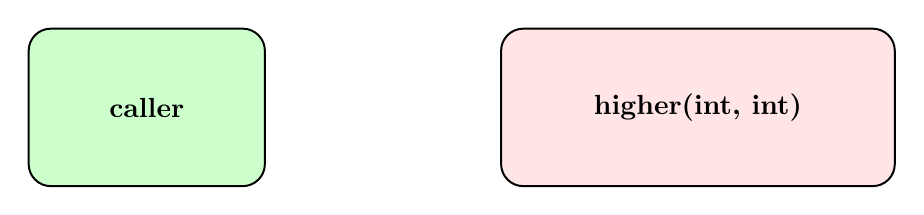
\begin{tikzpicture}
\draw [fill = green!20!white, rounded corners = 8pt, line width = 0.25mm]  (0,0) rectangle (3,2) node[pos=.5] {\textbf{caller}};
\draw [fill = red!10!white, rounded corners = 8pt, line width = 0.25mm]  (6,0) rectangle (11,2) node[pos=.5] {\textbf{higher(int, int)}};
\arrow{startX=3,startY=1,endX=6,endY=1, label=\textbf{\textcolor{red}{1, 5, 3}}}
\arrow{colour=red, arrowheadsize=0.01, startX=3,startY=2,endX=6,endY=-1, label=\textbf{too many parameters}, style=dashed, aboveBelow=below}
\arrow{colour=red, arrowheadsize=0.01, startX=3,startY=-1,endX=6,endY=2, style=dashed, aboveBelow=below}
\end{tikzpicture} \egroup


\vskip 2cm

Example 4

\vskip 2cm

\bgroup \tikzset{png export} 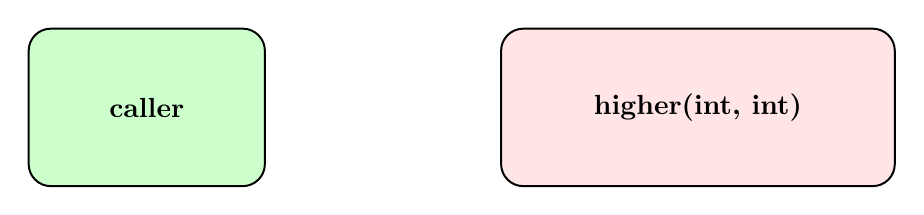
\begin{tikzpicture}
\draw [fill = green!20!white, rounded corners = 8pt, line width = 0.25mm]  (0,0) rectangle (3,2) node[pos=.5] {\textbf{caller}};
\draw [fill = red!10!white, rounded corners = 8pt, line width = 0.25mm]  (6,0) rectangle (11,2) node[pos=.5] {\textbf{higher(int, int)}};
\arrow{startX=3,startY=1,endX=6,endY=1, label=\textbf{\textcolor{red}{true}, 5}}
\arrow{colour=red, arrowheadsize=0.01, startX=3,startY=2,endX=6,endY=-1, label=\textbf{invalid type for first parameter}, style=dashed, aboveBelow=below}
\arrow{colour=red, arrowheadsize=0.01, startX=3,startY=-1,endX=6,endY=2, style=dashed, aboveBelow=below}
\end{tikzpicture} \egroup

\vskip 2cm

Syntax of a function is:

\begin{verbatim}
returnType function(	<parameters>) {
    <some code>
    <return statement>
    <some code>
}
\end{verbatim}

Example,

\begin{lstlisting}
boolean divisible(int a, int b) {
	if(a%b == 0)
		return true;
	else
		return false;
}
\end{lstlisting}

\begin{itemize}
	\item The function accepts two parameters, that it names \texttt{a} and \texttt{b} during the execution of the function. Here, \texttt{a, b} are called \textit{formal parameters}.
	\item The function returns a value of type \texttt{boolean} back to the caller.
	\item Let's say the call to function \texttt{divisible} is,

\begin{lstlisting}
int x = 7, y = 5;
boolean status = divisible(x+y, x-y);
\end{lstlisting}

	\item The integer expressions \texttt{x+y}  and \texttt{x-y} are evaluated to 12 and 2 respectively. The evaluated values are known as \textit{actual parameters} and are copied into the formal parameters \texttt{a, b} during the execution of \texttt{divisible(12, 2)}.
	
	\item Scope is transferred from the caller to the function call \texttt{divisible(12, 2)}. 
	
	\item The function determines that the boolean expression \texttt{a\%b == 0} is \texttt{true}, executes the if-block and returns \texttt{true}.
	
	\item The control is transferred back to the caller with the returned value \texttt{true} being copied into variable \texttt{status}.
\end{itemize}

\bgroup \tikzset{png export} 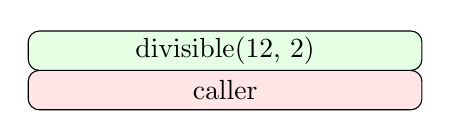
\begin{tikzpicture}
\scopeblock{functionName=caller,variables={{"x=7", "y=5", "status"}},width=3.2}
\scopeblock{x=6,functionName={divisible(12, 2)},variables={{"a = 12","b = 2"}},width=3.2}
\arrow{startX=3,startY=2.3,endX=5.5,endY=2.3}
\draw[rounded corners,fill=red!10!white] (10,0) rectangle (15,0.5) node[pos=.5] {caller};
\draw[rounded corners,fill=green!10!white] (10,0.5) rectangle (15,1) node[pos=.5] {divisible(12, 2)};
\end{tikzpicture} \egroup

\bgroup \tikzset{png export} 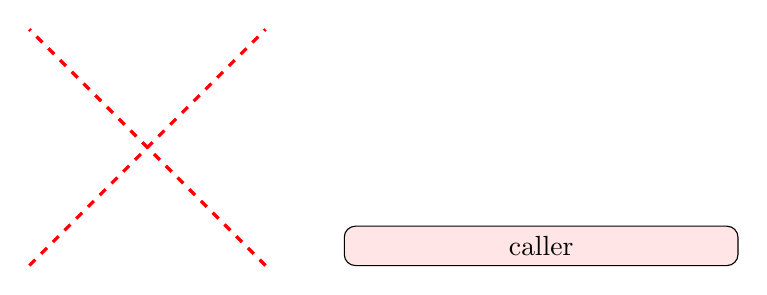
\begin{tikzpicture}
\scopeblock{functionName=caller,variables={{"x=7", "y=5", "status=true"}},width=3.2}
\scopeblock{x=6,functionName={divisible(12, 2)},variables={{"a = 12","b = 2"}},width=3.2}
\arrow{startX=5.5,startY=2.3,endX=3,endY=2.3, style=dashed, label=\textbf{true}}
\draw[rounded corners,fill=red!10!white] (10,0) rectangle (15,0.5) node[pos=.5] {caller};
\draw[dashed, very thick, red](6, 0) -- (9,3);
\draw[dashed, very thick, red](9, 0) -- (6,3);
\end{tikzpicture} \egroup

\end{document}
